\documentclass[../../../../projectPlan.tex]{subfiles}

\begin{document}

	\section{Project Effort and Cost}

		To make an Effort estimation we have to compute this formula:

		\[effort = 2.94 * EAF * (SLOC/1000)^E\]

		Where:
		\begin{itemize}
			\item \(effort\) is the value to estimate.
			\item \(2.94\) is a constant defined by COCOMO II 2000.0.
			\item \(EAF\) is the "Effort Adjustement Factor" calculated in the following sections.
			\item \(SLOC/1000\) that is the KSLOC (Kilo SLOC) number.
			\item \(E\) that is an exponent calculated in the following sections.
		\end{itemize}

		\subsection{Computation of \(E\) parameter}
			The parameter \(E\) is calculated as:
			\[E = B + 0.01 * SFs\]
			Where:
			\begin{itemize}
				\item \(B\) is a constant given by the COCOMO II and his value is 0.91.
				\item \(SFs\) is an aggregation of five Scale Factors described in the document at \url{http://csse.usc.edu/csse/research/COCOMOII/cocomo2000.0/CII_modelman2000.0.pdf}
			\end{itemize}
			

			The following table contains the variuos values for these Scale Factors (table taken from the previous URL).

			\begin{figure}[H]
				\centering
				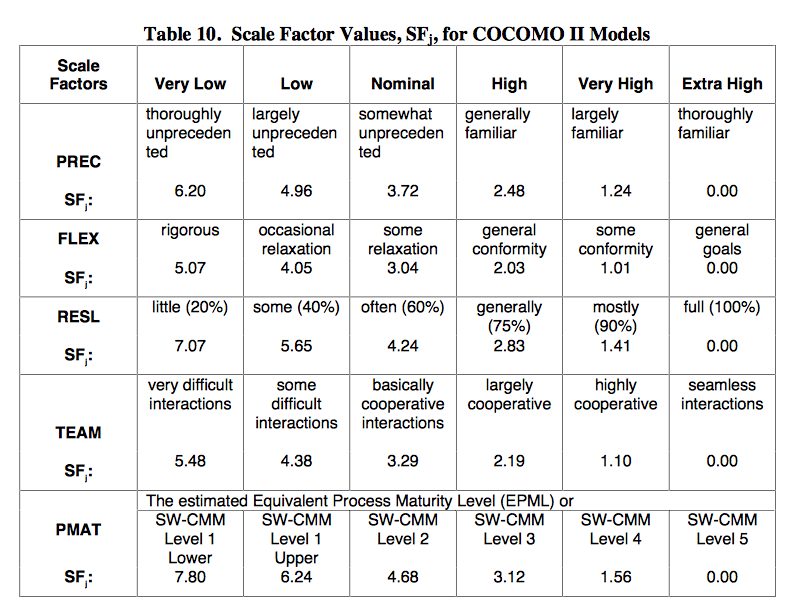
\includegraphics[width=\textwidth, scale=0.5]{../images/ftable.png}
			\end{figure}

			\begin{itemize}
				\item \textbf{PREC} (Previous experience of the organization with these type of projects): LOW (4.96).
				\item \textbf{FLEX} (Degree of flexibility in development process): HIGH (2.03).
				\item \textbf{RESL} (Risk Analysis): HIGH (2.83).
				\item \textbf{TEAM} (How well the development team knows each other): EXTRA HIGH (0.00).
				\item \textbf{PMAT} (Maturity of the Organization): NOMINAL (4.68).
			\end{itemize}

			The result is the sum of these factors:
			\[SFs = \sum_{j=1}^{5} SF_j = 14.67 \]

			So we can now compute the \(E\) parameter:
			\begin{align*}
				E & = B + 0.01 * SFs \\
			   	  & = 0.91 + 0.01 * 14.67 \\
			      & = 1.558
			\end{align*}

		\subsection{Computation of \(EAF\) parameter}
			All the parameters discussed in this paragraph are described in section 3.2 of the document at this URL: \url{http://csse.usc.edu/csse/research/COCOMOII/cocomo2000.0/CII_modelman2000.0.pdf}

			\begin{itemize}
				\item \textbf{Required Software Reliability (RELY)}
				      The results of a failure in our system is easily recoverable (e.g. loss of priority in the zone queues) so the RELY factor is LOW (count as 0.92).

				\item \textbf{Data Base Size (DATA)}
				      The effort needed to assemble and maintain the data required to complete test of the program is such that the DATA factor is NOMINAL (count as 1.00).

				\item \textbf{Product Complexity (CPLX)}
				      The area of our project is "Data Management" and the complexity is HIGH because we have simple triggers activated by data stream contents and complex data restructuring (e.g. maintain the zone queues updated) (count as 1.17).
				
				\item \textbf{Developed for Reusability (RUSE)}
				      This factor accounts for the additional effort needed to construct components intended for reuse on current or future projects. We think that we only have to design modules for the internal reuse in the myTaxiService system, so the descriptor is: NOMINAL (count as 1.00).
				
				\item \textbf{Documentation Match to Life-Cycle Needs (DOCU)}
				      We think that the documentation we have to produce is necessary in function of the lifecycle of the system, so we assign to DOCU the NOMINAL level (count as 1.00).
				
				\item \textbf{Execution Time Constraint (TIME)}
				      Our system is supposed to be fast because it's a Taxi reservation system, so the system is supposed to occupy less than 50 percent of the available execution time.
				      The label for TIME is NOMINAL (count as 1.00).
				
				\item \textbf{Main Storage Constraint (STOR)}
				      Due to the fact that the web application does not occupy the user's memory and that the mobile application is relatively simple, we only have to consider the memory occupation on the server side. This memory occupation change in function of the number of the users and increments if the usage of the system is high. We have to consider many things like Server Software, External API implementation, Database Space, so the label for TIME is HIGH (count as 1.05).
				
				\item \textbf{Platform Volatility (PVOL)}
				      Due to the fact that we have to implement a Mobile Application and a Web application, and the technologies we have to use (Android, iOS, Windows Phone programming languages, JS Frameworks for the website) receives continuous updates, we have to consider the PVOL facor at least NOMINAL (count as 1.00).
				
				\item \textbf{Analyst Capability (ACAP)}
				      Through the designing of the project, the team has collaborated, designed and analyzed every different scenarios for the application.
				      There is a VERY HIGH rating for the ACAP factor (count as 0.71).
				
				\item \textbf{Programmer Capability (PCAP)}
				      Another time, the development team (that is the project management team) is heavily skilled in cooperation and communication because we have developed other projects with great results. The rating for PCAP is VERY HIGH (count as 0.76).
				
				\item \textbf{Personnel Continuity (PCON)}
                      Since we are the only two persons at work on this project, we does not count PCON as a factor that determines the \(EAF\) parameter (FULL continuity is EXTRA HIGH and it has no coefficient).
				
				\item \textbf{Applications Experience (APEX)}
                      Since we have developed another project for 6 months we have a LOW level for the APEX factor (count as 1.10).
				
				\item \textbf{Platform Experience (PLEX)}
                      We have experience in using Databases, building GUIs and developing distributed systems and we have worked with these structures for more than 6 months. But since our experience is not the same in every subject, we prefer to set the PLEX factor as LOW (count as 1.09).

				\item \textbf{Language and Tool Experience (LTEX)}
				      Our team is skilled in development and designing OO applications and Distributed systems. But we are not so much skilled in building the Documentation (Requirements Analysis, Project Plan, Integration Test Documents, etc...) so we prefer to set the LTEX factor as NOMINAL (count as 1.00).

				
				\item \textbf{Use of Software Tools (TOOL)}
				      All the tools we have used are for the design of the application (Lifecycle tools) and for development (Code \& Edit) so we have to set TOOL factor to NOMINAL (count as 1.00). 
				
				\item \textbf{Multisite Development (SITE)}
				      The team is composed by two persons, we live at a distance of about 10 Kilometers, we have worked in the same place for the entire duration of the project enabling the direct communication between us. The SITE factor is set to EXTRA HIGH (count as 0.80).
				
				\item \textbf{Required Development Schedule (SCED)}
				      We have a fair distribution of time thanks to the things discussed in SITE factor.
				      So we can set SCED factor as NOMINAL (count as 1.00)

			\end{itemize}

			Now, given these factors we can define the set of factors:

			\begin{align*}
			    F = \{ & RELY, DATA, CPLX, RUSE,\\
			          & DOCU, TIME, STOR, PVOL,\\
			          & ACAP, PCAP, PCON, APEX,\\
			          & PLEX, LTEX, TOOL, SITE, SCED \}
		    \end{align*}

		    and we can define a generic element of the \(F\) set as:

		    \begin{center}
		    	\(f_i\) such that \(i=1,2,...,|F|\)
		    \end{center}

		    So the final \(EAF\) parameter can be computed as:

		    \[EAF = \prod_{i=1}^{|F|} f_i = 0.585\]

		\subsection{Effort and Duration}

			Now thate we have successfully computed the \(EAF\) and the \(E\) parameters, we can now apply the \(effort\) estimation function, considering the Java implementation:

			\begin{align*}
				effort & = 2.94 * EAF * (SLOC_java/1000)^E
                       & = 2.94 * 0.585 * (4823/1000)^1.558
                       & = 19.96 PM
			\end{align*}

			Since the Number of Persons (\(N_{persons}\)) that has to be assigned to the project is calculated as:

			\[N_{persons} = effort / projectDuration \]

			We can exploit this formula (since the team has a fixed \(N_{persons} = 2\)) and calculate how much time the team needs to develop the entire system:

			\begin{align*}
				projectDuration & = effort / N_{persons}
				                & = 19.96 / 2
				                & = 9.98\ months\ (10\ months)
			\end{align*}
\end{document}